%!TEX TS-program = xelatex
\documentclass[main]{subfiles}
%这是一个子文件,单独编译时会自动导入main文件的导言区
%这里可以放自定义命令,不会和别人的冲突请放心
%但是不能放newtheorem等高级命令,需要请在群里说
%下面是一些数学命令的简化,可以保留,可以删去,也可以按你的习惯修改
\usetikzlibrary{arrows.meta}
\usetikzlibrary{positioning}
\def\e{\textup{e}}
\def\i{\textup{i}}
\def\dif{\textup{d}}
\def\T{\textup{T}}
\def\diag{\textup{diag}}
\def\id{\textup{id}}
\newcommand{\toi}[1]{{#1}\to\infty}
\newcommand{\dis}{\displaystyle}
\newcommand{\bv}{\mathrm{BV}}
\newcommand{\ac}{\mathrm{AC}}
\newcommand{\mr}{\mathbb{R}}
\newcommand{\mn}{\mathbb{N}}
\newcommand{\mq}{\mathbb{Q}}
\newcommand{\mz}{\mathbb{Z}}
\newcommand{\rel}{\text{ rel }}
\newcommand{\sgn}{\operatorname{sign}}
\newcommand{\ve}{\varepsilon}
\newcommand{\bs}{\backslash}
\newcommand{\Span}{\operatorname{span}}
\renewcommand{\ll}{\lim\limits}
\renewcommand{\ker}{\operatorname{Ker}}
\renewcommand{\hom}{\operatorname{Hom}}
\renewcommand{\leq}{\leqslant}
\renewcommand{\geq}{\geqslant}
\begin{document}
\renewcommand{\filename}{费马大定理}%在这里填你的文件名,避免\label冲突
%这里开始写你的代码
\section{费马大定理}
\subsection{猜想提出}
毕达哥拉斯定理说的是: 直角三角形两直角边平方之和等于斜边平方, 即$x^2+y^2=z^2$ 。公元前12世纪我国《周髀算经》也提出过“勾三股四弦五”, 后称勾股定理。
\par 那$x^n+y^n=z^n (n > 2)$ 有无正整数解? 这个问题的提出和“解答”始于法国业余数学家费马。1637年,在《算术》副本的空白处, 费马写到: “ 一般地将一个高于二次的幂分成两个同次幂之和,这是不可能的。关于此,我确信我发现一种美妙的证法,可惜这里的空白处太小,写不下 。” 
就是费马的糊弄的这句话, 开启了全世界数学家们358年的证明历程。

\begin{figure}[H]
	\centering
	\subfloat [费马大定理纪念邮票]
	{
		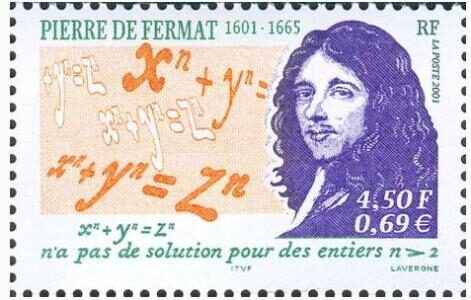
\includegraphics[width=0.20\textwidth]{0.jpg}
		 %\caption{以费马定理为主题的纪念邮票}
	}
	\subfloat [安德鲁·怀尔斯]
	{
		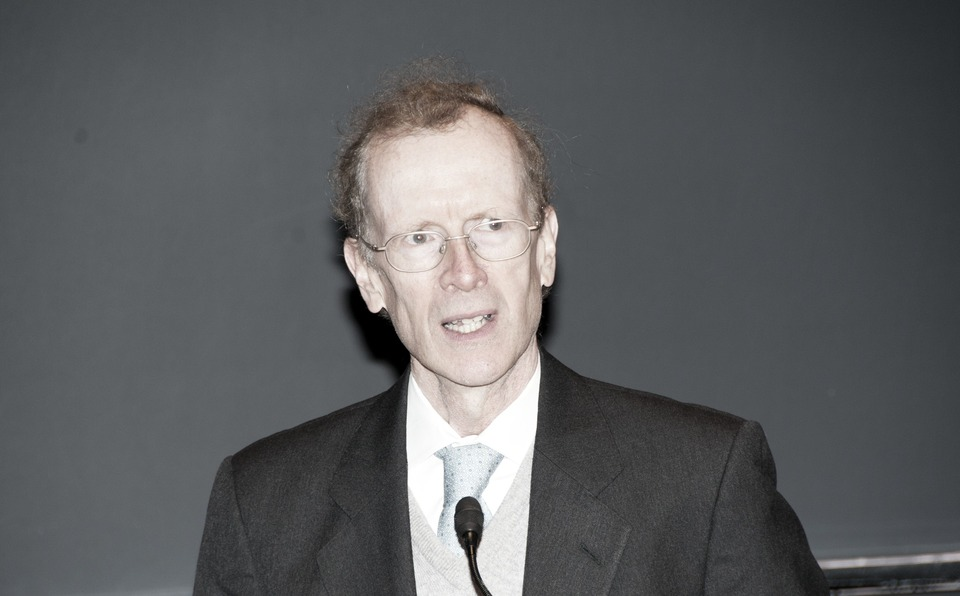
\includegraphics[width=0.20\textwidth]{0 (1).jpg}
	}
\end{figure}
\subsection{定理叙述}
\begin{theorem}[费马大定理]
当整数 $ n>2$ 时, 下述关于 $x,y,z$ 的不定方程无正整数解
\[ x^n + y^n = z^n\]
\end{theorem}
\subsection{证明历程}
委员会收到数千个不正确的证明, 所有纸张叠加达到约10英尺(3米)的高度
\par 1637年, 数学家根据费马的少量提示用无穷递降法证明了 $n=4$ 的情况。
\par 1770年, 欧拉证明了$n=3$的情况。
\par 1825年, 索菲·日耳曼证明了$n=5$的情况, 她引进了一些新的方法, 可以推广到很多素数
\par 1847年, 加布里埃尔·拉梅基于 $x^p + y^p = z^p$ 在复数域内的分解给出一个伪证。库默尔将深入研究这种方法, 建立了 “理想数” 的理论, 解决了所有正规(regular)素数的情况。
\par 1983年, 格尔德·法尔廷斯证明莫德尔猜想。作为推论,对于给定的整数
$n>2$, 至多存在有限组互素的
$a,b,c$ 使得
$a^{n}+b^{n}=c^{n}$ 从无限到有限,前进了一大步。
\par 1986年, 格哈德·弗赖提出“$\epsilon-$猜想”并被证实: 若存在 $a,b,c$ 使 $a^n + b^n = c^n$ 则椭圆曲线 $y^2 = x (x-a^n)(x+b^n)$ 将是谷山-志村猜想的一个反例。联系了费马大定理与椭圆曲线, 模形式。
\par 1995年, 安德鲁·怀尔斯和理查·泰勒在一特例范围内(半稳定椭圆曲线)证明谷山志村猜想, 上述的椭圆曲线刚好在这一特例范围内, 从而证明费马大定理。
\par 怀尔斯证明的过程甚具戏剧性。他在不为人知(除了妻子)的情况下埋头苦干了7年, 然后于1993年6月宣布他的证明, 瞬即成为世界头条。但马上被检查出错误, 怀尔斯和他的学生泰勒之后用近一年时间尝试补救, 终在1994年9月以一个之前怀尔斯抛弃过的方法得到成功。

\subsection{重大意义}
怀尔斯说:“判断一个数学问题是否是好的,其标准就是看它能否产生新的数学,而不是问题本身。” 费马大定理就是这样的一个好问题: 库默尔在证明中发展的“理想数”理论促进了代数数论的发展,而安德鲁·怀尔斯的“修补式证明”,对代数几何、数论、调和分析、拓扑学等数学分支产生了深远的影响,在他的证明的基础下,谷山-志村猜想在4年后被证明。
\end{document}
